% v2-acmlarge-sample.tex, dated March 6 2012
% This is a sample file for ACM large trim journals
%
% Compilation using 'acmlarge.cls' - version 1.3, Aptara Inc.
% (c) 2011 Association for Computing Machinery (ACM)
%
% Questions/Suggestions/Feedback should be addressed to => "acmtexsupport@aptaracorp.com".
% Users can also go through the FAQs available on the journal's submission webpage.
%
% Steps to compile: latex, bibtex, latex latex
%
\documentclass[prodmode,acmtap]{acmlarge}

\makeatletter
\def\runningfoot{\def\@runningfoot{}}
\def\firstfoot{\def\@firstfoot{}}
\makeatother

%Metadata Information
\acmVolume{2}
\acmNumber{3}
\acmArticle{1}
\articleSeq{1}
\acmYear{2015}
\acmMonth{12}

\newcommand*{\myalign}[2]{\multicolumn{1}{#1}{#2}}


% Package to generate and customize Algorithm as per ACM style
\usepackage[ruled]{algorithm2e}
\usepackage{caption}
\usepackage{amsmath}
\usepackage{subcaption}
\usepackage{wrapfig}
\usepackage{textcomp}
\captionsetup{compatibility=false}
% \usepackage{mathtools}
\SetAlFnt{\algofont}
\SetAlCapFnt{\algofont}
\SetAlCapNameFnt{\algofont}
\SetAlCapHSkip{0pt}
\IncMargin{-\parindent}
\renewcommand{\algorithmcfname}{ALGORITHM}

% Page heads
% \markboth{D. Pineo, C. Ware and S. Fogarty}{Neural Modeling of Flow Rendering Effectiveness}

% Title portion
\title{What's cooking. STAT 841 final report.}
\author{Sajin Sasy and Alexandra Vtyurina \affil{University of Waterloo}
} 
% NOTE! Affiliations placed here should be for the institution where the
%       BULK of the research was done. If the author has gone to a new
%       institution, before publication, the (above) affiliation should NOT be changed.
%       The authors 'current' address may be given in the "Author's addresses:" block (below).
%       So for example, Mr. Fogarty, the bulk of the research was done at UIUC, and he is
%       currently affiliated with NASA.

\begin{abstract}
The paper describes the approach that we took for the Kaggle competition of identifying recipe cuisines based on the list of their ingredients. We provide detailed description of how we tackled the problem of data cleaning and what approaches for classification we chosen and why. We also report on the results and provide a justification for them. 

\end{abstract}


\begin{document}

% \begin{bottomstuff}
% This work is supported by the Widget Corporation Grant \#312-001.\\
% Author's address: D. Pineo, Kingsbury Hall, 33 Academic Way, Durham,
% N.H. 03824; email: dspineo@comcast.net; Colin Ware, Jere A. Chase
% Ocean Engineering Lab, 24 Colovos Road, Durham, NH 03824; email: cware@ccom.unh.edu;
% Sean Fogarty, (Current address) NASA Ames Research Center, Moffett Field, California 94035.
% \end{bottomstuff}


\maketitle

% Head 1
\section{Introduction}
This report is describing the approach taken and results achieved in Kaggle\footnote{https://www.kaggle.com/} competition called ``What\textquotesingle s cooking''\footnote{https://www.kaggle.com/c/whats-cooking}. The evaluation was performed using a dataset provided by Yummly\footnote{http://www.yummly.com/} -- a popular culinary website. Two datasets - training and testing were given to the participants of the competition. Kaggle platform allowed participants submit their results 5 times every 24 hours. 

While working on this project we have faced several challanges. First of all, the data provided could be interpreted in multiple different ways. We talk about data analysis in more details in the \textit{Data munging} section. Second of all, we found that some cuisines have a very tightly overlapping list of ingredients in their recipes. Our assumption was that it was due to their close geographical proximity, as well as cultural influences. For example, we found that thai and vietnamese cuisines use similar sets of ingredients. 

We have taken several classification approaches and compared their results. In particular, we used linear SVM, logictic regression and random forests. We found that linear SVM was performing the best for the given problem. We also used different tuning techniques to increase the accuracy. For example, we tried one versus one model, as well as one versus all. One versus all model yeilded high precision results, but very low recall, which was due to large overlap between classes. The detailed description of the approahces we have tried is in the \textit{Classification approaches} section. 

The \textit{Experiments} section provides results we got for different data interpretation models and classification techniques. We also provide justification for the results obtained. Finally, we conclude with the general discussion and potential future work that could be done to enhance current results. 

\section{Related work}
The problem of recipe classification is not the most popular, to the best of our knowledge. UbiComp people tackled a very similar problem, using a different dataset \cite{ubicomp}. The research community is more active in the field of culinary recommendation systems and their ingredients nutrition \cite{nutrition}.


\section{Data analysis}
Kaggle provided all participants with two sets of data -- training and testing. Training data included almost 40 thousand recipes encoded as a list of json objects. Every recipe consisted of the following fields: \textit{id}, \textit{cuisine}, \textit{ingredients}. 20 different cuisines with 6714
%(without splitting, 3065 with splitting no stemming, 2692 with splitting and stemming) 
unique ingredients were presented in the training dataset. The test data had the same format with the exception of the \textit{cuisine} label, that should be predicted. The expected format of submission was a csv file with two columns - \textit{recipe id} and its predicted \textit{cuisine label}.

\begin{wrapfigure}{l}{0.5\textwidth}
  \begin{center}
    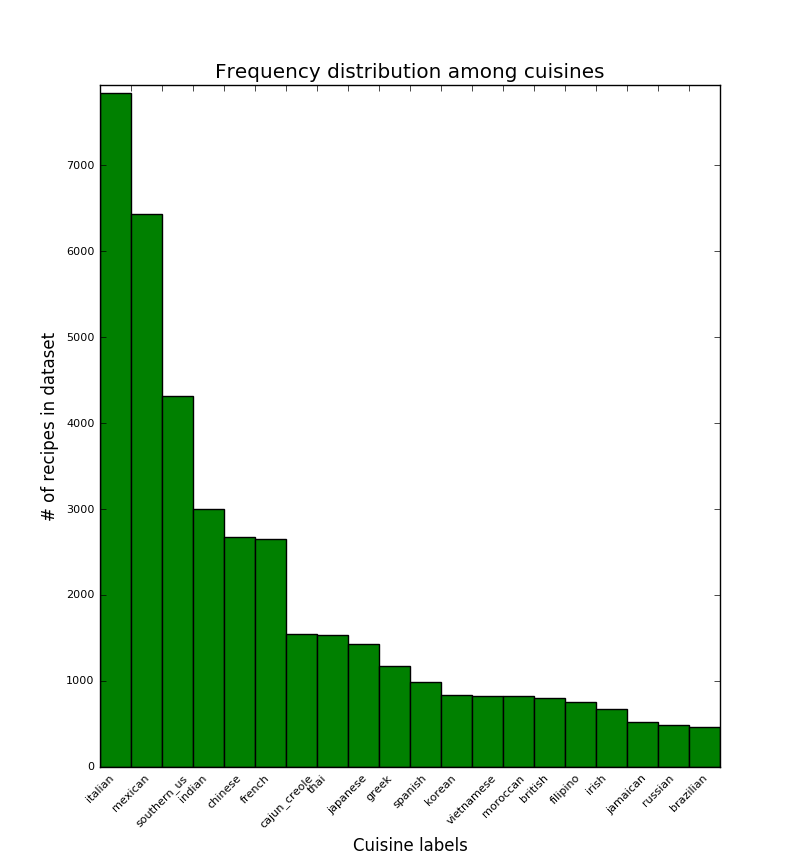
\includegraphics[width=0.48\textwidth]{cuisine_freq_hist_green_wlabels}
  \end{center}
  \caption{Training data is unbalanced. Italian and mexican recipes dominate, whereas brazilian and russian are underrepresented.}
\end{wrapfigure}

The training data provided was quite rich however unbalanced. Figure \ref{cuisine_freq} shows how many recipes for each type of cuisine are contained in the training dataset. Underrepresented classes include brazilian, russian, jamaican, etc and contain under 800 recipes, whereas italian recipes dominate. 

It is worth mentioning the variability of the ingredients representation. Some only consisted of a single word (for ex. ``tomatoes''), whereas others contained multiple words (for ex. ``ground black pepper''). Moreover some ingredients also included attributes, such as ``2 large eggs'' and brand names ``Sargento® Traditional Cut Shredded Mozzarella Cheese''. This variability introduced additional noise to the data, and prevented us from using each ingredient as a separate feature. We further elaborate on the topic of data cleaning. 

\subsection{Data munging}
Given that ingredients may contain multiple words, using each ingredient as a separate feature will introduce a lot of noise, as “egg” and “eggs” will be considered two different features. Prior to classifying recipes, we cleaned the data in several different ways to see which one yields the best results and removes the most of noise. We chose different approaches, starting with a very mild one and building on top of one another to eventually reach the strictest cleaning strategy. 
We started off by splitting each ingredient into words\footnote{We used NLTK built in tokenizer to tokenization} and using them as features. This approach could deal with ingredients like ``large egg'' and ``egg'', splitting ``large egg'' into ``large'' and ``egg'', after which we had two ``egg'' terms match. 
But we still had problems in cases of ``three large eggs'' and ``egg'', where after splitting ``three large eggs'' into ``three'', ``large'', ``eggs'', the terms ``eggs'' and ``egg'' were still considered to be different. Stemming terms\footnote{We used Porter stemmer providd by NLTK} after splitting would solve this problem by transforming ``eggs'' into ``egg''. 

After examining the data we found that there are now ingredients that don’t add to the flavour of the dish, for example ``three'' and ``large'' (from ``three large eggs''), or ``ground'' and ``black'' (from ``ground black pepper''). Our assumption was that the main difference between cuisines comes from their flavour, hence only the ingredients themselves matter, rather than their modifiers. We wanted to remove modifiers based on the results of POS tagging (after manually examining the data we assumed that the majority of ingredients were nouns), but after performing POS tagging we found that the accuracy was extremely low due to the lack of context. E.g. we could only provide separate words and phrases to the tagger as opposed to entire sentences. As a result ingredients like ``store bought low sodium chicken broth'' the word ``store'' was considered a noun, even though it did not contribute to the flavour of the dish. Because of this issue we had to refuse from POS tagging and could not shrink initial data to bare ingredients. 


% \begin{figure}[tp]
% \centering
% 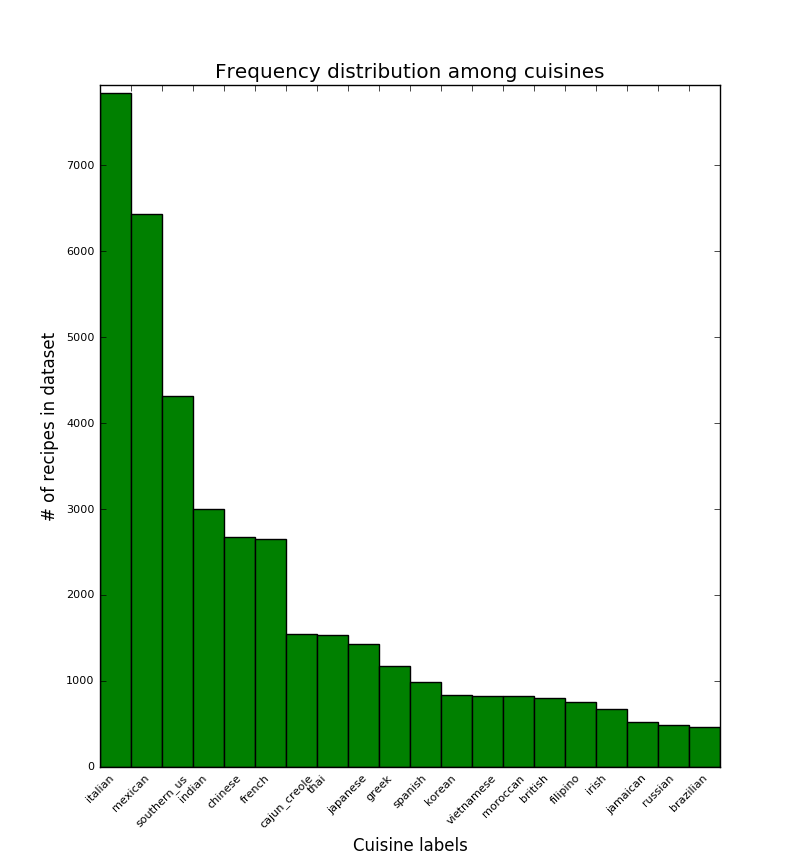
\includegraphics[scale=0.4]{cuisine_freq_hist_green_wlabels}
% \caption{Training data is unbalanced. Italian and mexican recipes dominate, whereas brazilian and russian are underrepresented.}
% \label{cuisine_freq}
% \end{figure}

\section{Feature selection}
While working with bigrams and trigrams, the number of features drastically increase as it would account for all potential two ingredient combinations over the feature space ( of 6640 ingredients). 
We used 5-fold cross validation to pick a bound on the number of features ( as shown in the graphs ) to use, rather than arbitrarily limiting it to a fixed number of features, where in by increasing features and comparing the change in cross-validation accuracy, we limited the features at a point where the cross-validation results were not improving and rather stagnating and/or decreasing with increase of features.

\begin {table}
\centering
\begin{tabular}{|r|l||r|l|}
  \hline
  Confused cuisines & num of recipes & Confused cuisines & num of recipes \\
  \hline
  Thai and Vietnamese & 31 & Chinese and Korean & 14\\
  Southern US and Cajun creole & 28 & Italian and Greek & 11\\
  Italian and French & 25 & Indian and Moroccan & 9 \\
  \hline
\end{tabular}
\caption{Some of the recipes were classified as multiple cuisines. The table shows cuisines that were confused most often.}
\label{confusiontable}
\end {table}

\subsection{PCA story}
After applying one-vs-one SVM to classify recipes we wanted to see how different the results would be for one-vs-all technique. For that we built 20\footnote{Same as the number of presented cuisines} hyperplanes to separate every single cuisine from the rest of the recipes. In this section we discuss our findings. 

\begin{figure}[hb]
\centering
\begin{minipage}{.45\textwidth}
  \centering
  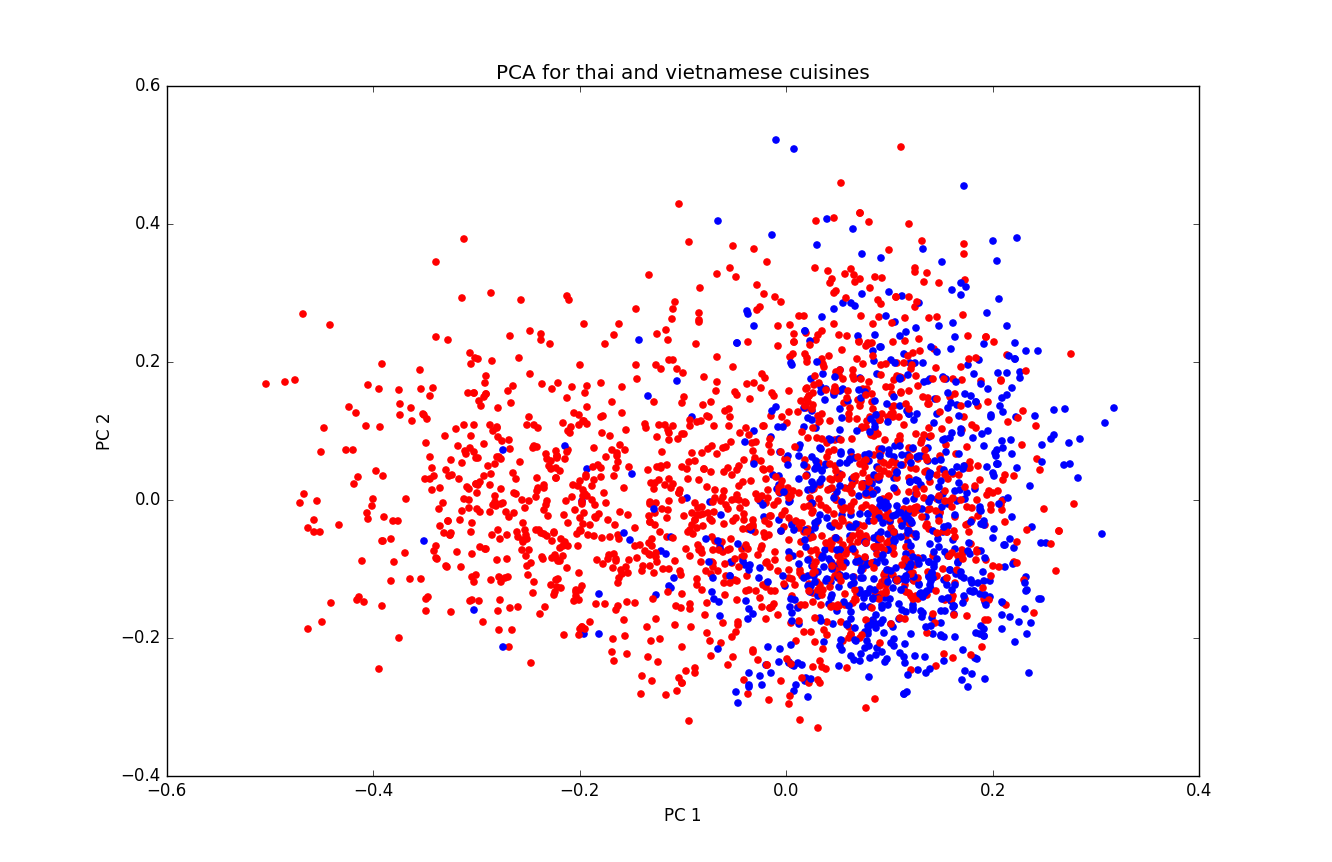
\includegraphics[width=\textwidth]{PCA_thai_vietnam}
  \captionof{figure}{The first and the second principal components for recipes of Thai and Taiwanese cuisines. Red points belong to Thai cuisine, blue points belong to Taiwanese cuisine.}
  \label{thai_taiwan_pca12}
\end{minipage}
\hfill
\begin{minipage}{.45\textwidth}
  \centering
  \includegraphics[width=\textwidth]{PCA_french_italian}
  \captionof{figure}{The first and the second principal components for recipes of french (red) and italian (bblue) cuisines.}
  \label{french_italian_pca12}
\end{minipage}%
\end{figure}

\begin {table}[t]
	\centering
	\begin{tabular}{|p{5cm}|p{5cm}|}
		\hline
		\myalign{|c|}{Negative components} & \myalign{c|}{Positive components}\\
		\hline
		\multicolumn{2}{|c|}{
		Terms in italics have been noted by cooking enthusiasts as typical  for} \\
		\myalign{| c }{thai cuisine} & \myalign{c|}{vietnamese cuisine}\\
		\hline
		past, lime, breast, bell, curri, light, unsweeten, skinless, boneless, thai, red, green, \textit{kaffir}, broth, stock, mushroom, 
		\textit{lemongrass}, chicken, \textit{coconut}, milk & \textit{mint}, garlic, white, vinegar, soy, pork, water, cucumb, black, 
		\textit{rice}, \textit{lettuc}, \textit{noodl}, sauc, peanut, sugar, beansprout, carrot, sesam, roast, egg \\
		\hline

	\end{tabular}

\caption{These ingredients contribute the most to the 1 principal component of the dataset comprised of thai and taiwanese recipes.}
\label{thai_taiwan_PC1}
\end {table}

\begin {table}[t]
	\centering
	\begin{tabular}{|p{5cm}|p{5cm}|}
		\hline
		\myalign{|c|}{Negative components} & \myalign{c|}{Positive components}\\
		\hline
		chocol, unsalt, milk, larg, sugar, butter, bake, egg, yolk, almond, vanilla, water, whip, confection, heavi, allpurpos, powder,
		flour, cream, extract & oregano, garlic, black, basil, extravirgin, chees, parmesan, oil, oliv, leav, tomato, pepper, 
		dri, clove, fresh, parsley, ground, red, onion, crush \\
		\hline

	\end{tabular}

\caption{These ingredients contribute the most to the 1 principal component of the dataset comprised of italian and french recipes. The separation is not between cuisine, but between deserts and main dishes}
\label{italian_french_PC1}
\end {table}

First of all, to use one-vs-all approach we had to reduce the original problem to a binary classification problem. We did it by constructing a separate dataset for every given cuisine, where we changed labels to 1, in case the recipe belonged to the currently chosen cuisine, and 0 otherwise. For example, for separating italian recepies we created a dataset, where a label was 1, if the recipe was originally italian, and 0 otherwise. 


Having done that for each of the 20 cuisines we used 5-fold cross validation to evaluate the accuracy of the new model\footnote{Considering that we were looking at a single cuisine at a time, we could not submit to Kaggle to test the accuracy}. We found that even though the reported accuracy was very high (it varied from 94\% to 99\% for different cuisines), some recipes did not have any label by the end of the classification, which means they were not classified as positive for any of the cuisines. From that we can conclude the recall was low, e.g. the proposed model was failing to identify all the recipes from a given cuisine. 

We have also found that few of the recipes were classified as positive for multiple cuisines. Table \ref{confusiontable} shows the list of cuisines that were confused most often and the number of recipes that were positively classified multiple times. As seen in the table the cuisines that get misclassified also share geographical location and/or cultural features. 



After we found that some cuisines are hard for SVM to separate we looked at their recipes more closely and tried to find distinct features that could be used to differentiate the cuisines. We performed PCA on the recipes of Thai and Vietnamese cuisines. As showm in figure \ref{thai_taiwan_pca12}, the overlap between the two cuisines is quite large and the separation is more clear alomg the first principal component. We extracted the terms that contributed the most to the first PC. For that we considered the values with the largest magnitude. Table \ref{thai_taiwan_PC1} shows the ingredients that contributed the most to the first principal component. As we can see, it does not show the clear separation between the cuisies, however, having studied some typical features of Thai food, we found that some of the products from the table are typical from Thai (left) anf Vietnamese (right) cuisines (such products are in italics). However if we perform the same amalysis for French and Italian cuisines, we can see in Table \ref{italian_french_PC1} that the first principal component separates types of dishes (desert from main dishes) rather than cuisines themselves. 







% \begin{figure}[tp]
% \centering
% 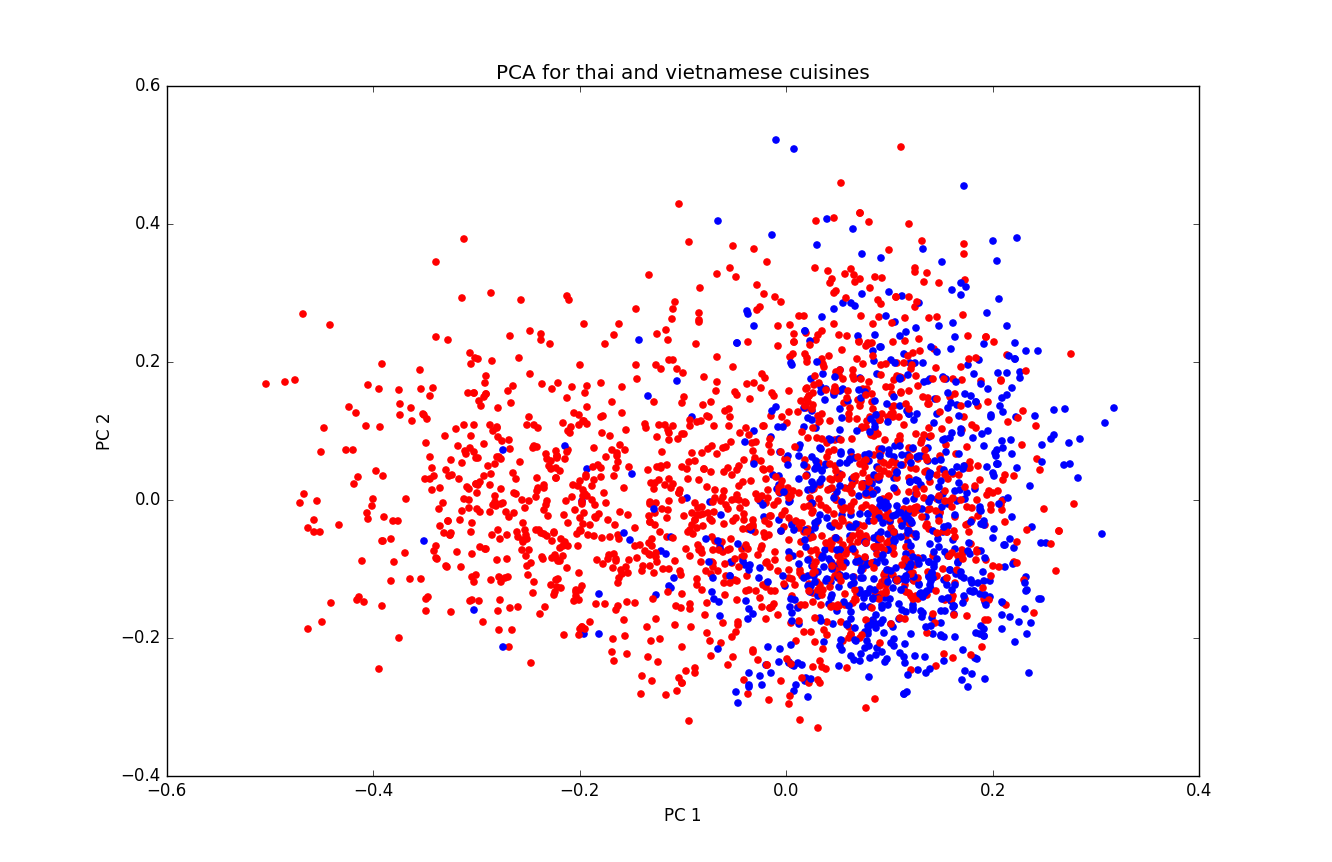
\includegraphics[scale=0.2]{PCA_thai_vietnam}
% \caption{The first and the second principal components for recipes of Thai and Taiwanese cuisines. Red points belong to Thai cuisine, blue points belong to Taiwanese cuisine.}
% \label{thai_taiwan_pca12}
% \end{figure}


\begin{figure}
\centering
\begin{minipage}{.45\textwidth}
  \centering
  \includegraphics[width=\textwidth]{bigrams}
  \captionof{figure}{Accuracy on training set (blue) and testing set (red) with variyng number of features. Features included unigrams (single terms) and bigrams(combinations of two terms)}
  \label{bigrams}
\end{minipage}%
\hfill
\begin{minipage}{.45\textwidth}
  \centering
  \includegraphics[width=\textwidth]{unigrams}
  \captionof{figure}{Accuracy on training set (blue) and testing set (red) with variyng number of features. Single terms were used as features.}
  \label{unigrams}
\end{minipage}
\end{figure}





\section{Classification approaches}
Since ``What\textquotesingle s cooking'' is a multi-class classification problem with an inherent input structure of the bag-of-words model, intuitively it would make sense to use a naive Bayes which fits well into both the structure of the underlying problem as well as the input format. However certainly naive Bayes is unlikely to produce a strong classifier as opposed to multiclass logistic regression or SVM.

The classification method involved has to make judgements based on the presence of ingredients in a given recipe. This suggests a quite simple model of classification, intuitively the cuisine that a recipe belongs to would be based on just the presence or absence of an ingredient from the feature list of ingredients, hence suggesting a simple linear model of classification as opposed to a more complicated model like Neural Networks which would be more prone to overfitting in such an instance. 

\subsection{Support Vector Machine}

As opposed to other linear classifiers, the primary distinction that sets SVM aside is the fact that 
produces a max-margin hyperplane to separate the data points , in contrast other models would produce one among the infinite number of hyperplanes that could separate them (and this applies even in the case of data that is not linearly separable). Simply by concept itself, the notion of a classifier that produces the maximum margin between two classes would intuitively produce a better classifier as opposed to the others, and we were certain that this would be the ideal method for classification for our problem at hand.

The key advantage of using Support Vector Machine for us lie in its robustness to overfitting and it’s ability to produce a max-margin hyperplane. Just as we had expected our best results came from the SVM classifier itself. The only setback of SVM is that it is inherently a binary classifier, so we would have to use it in our problem either by using  it as a one-vs-all or as a set of one-vs-one classifiers for every pair of cuisines. 

For implementing it we made use of svm.SVC package of exposed in sklearn package for Python, which in itself is based on libsvm \cite{scikitsvc}. We tuned the SVM model to try both one-vs-one and one-vs-all to see that one-vs-one was indeed producing slightly better results (as seen in the Table \ref{resultstable}) . 

\subsection{Random Forests}

As opposed to other linear models, we decided to use Random Forest, which is generally classified as an ensemble technique, since in effect it performs majority vote with a large number of decision trees used to estimate the value of the function. Since the underlying technique is actually of decision trees, one major advantage is that it is no longer bound to linearity, in the sense that it would not try to model based on linearity of features and would intuitively do well for binary features (like the bag-of-words). Another significant advantage is that random forests work in synchrony with bootstrap aggregating or bagging, as since each of the constituent decision trees can be trained with bootstrapped training sets, and this is a good mechanism for checking overfitting


\section {Experiments}
We initially started experimenting with Naive Bayes, and the results were not promising just as what we had expected and as seen from the table. Logistic regression on the other hand produced good results, and this is justified as multi-class logistic regression uses maximum likelihood for estimation which would maximize the probability of a data point belonging to a particular cuisine given the likelihood for the underlying distribution of features to do so.

After we hit a wall with data munging techniques and our aforementioned classifiers, we wanted to experiment with boosting as it seemed like the next step to further refine our classifier without easily exposing it to the risk of overfitting. We worked with xgboost (extreme gradient boosting) to compare the results of boosting in our problem with our results, we used boosting with logistic regression model for the aforementioned results.

\begin {table}
	\centering
	\begin{tabular}{|l|c|}
		\hline
		\myalign{|c|}{Model} & \myalign{|c|}{Score} \\ 
		\hline
		SVM ( linear kernel , using bigrams , one-vs-one model) & \textbf{0.79053} \\
		\hline
		SVM ( linear kernel , one-vs-one model ) & 0.78831 \\
		\hline
		SVM ( linear kernel , using bigrams , one-vs-all model) & 0.78761 \\
		\hline
		Logistic Regression & 0.78309 \\
		\hline
		SVM ( linear kernel , one-vs-all model) & 0.77253 \\
		\hline
		Boosting ( xgboost ) & 0.76760 \\
		\hline
		Random Forests (with 100 trees and Bootstrap) & 0.74361\\
		\hline
		Naive Bayes & 0.66814 \\
		\hline
		Experimental Ensemble Technique\footnote{The detailed description of the technique is given in the \textit{Discussion} section} & 0.79133 \\
		\hline		

	\end{tabular}

\caption{ The results of different approaches after submitting to Kaggle.}
\label{resultstable}
\end {table}

\section{Discussion}
We refrained from Word2Vec, primarily because the purpose it serves does not match the classification task that was at hand. Word2Vec is extremely efficient in semantic analysis of words in a corpus (provided it is trained with a large enough training corpus), however in an ingredient based recipe classification there is not much room for semantic analysis of the ingredients.

We even experimented with our own ensemble technique using SVM\textquotesingle s by initially using individual one-vs-all SVM\textquotesingle s to classify data points in our training set, and then reclassifying the data points that either mapped to no classes or multiple classes under the one-vs-all SVM\textquotesingle s, using the best results for these data points from a one-vs-one SVM classifier. The underlying objective and intuition was to separate data points that were able to be classified well from the other data points that were more significantly ambiguous in their classifications. Surprisingly enough, this produced our best result although by a marginal difference, hence there is still scope for some improvisation on this so as to analyze the ambiguously classified points in a better fashion.


\section{Conclusion}
In this report we tackled the problem of recipe classification based on their ingredients. We worked on the dataset provided by Yummly, and evaluated the results using Kaggle platform. The problem has been shown to be challenging due to the variery of ingredients used in different cuisines and their overlapping nature. We tried tokenization and stemming of the multiwords ingredents, as well as using a list of attributive words (large, store-bought, etc), that did not add to the flavour of the dish. The latter has been shown to yeild better results. However there is still room for improvisation, since many ingredients in the data sets have extremely different supporting prefix and suffix words, and this gives rise to an NLP challenge in extracting the essential components of an ingredient over generalizing or losing out on too much information. We applied several techniques for classification and found SVM to be the most suitable for this particular competition.

% Bibliography
\begin{thebibliography}{1}

  \bibitem{ubicomp} Su, Han and Lin, Ting-Wei and Li, Cheng-Te and Shan, Man-Kwan and Chang, Janet {\em Automatic Recipe Cuisine Classification by Ingredients},  UbiComp 2014 Adjunct.
\\
  \bibitem{scikitsvc} Chang, Chih-Chung and Lin, Chih-Jen, {\em LIBSVM: A Library for Support Vector Machines}, ACM Trans. Intell. Syst. Technol. April 2011
\\

  \bibitem{svm} Corinna Cortes and Vladimir Vapnik {\em Support-vector networks}, Machine Learning 1995
 \\

  \bibitem{nutrition} Ueta, Tsuguya and Iwakami, Masashi and Ito, Takayuki {\em A Recipe Recommendation System Based on Automatic Nutrition Information Extraction}, KSEM 2011 


\end{thebibliography}

\end{document}
% End of v2-acmlarge-sample.tex (March 2012) - Gerry Murray, ACM
